\documentclass[sutton_barto_notes.tex]{subfiles}

\begin{document}


\newpage
\section{n-step Bootstrapping}

\begin{itemize}
\item unify the MC and one-step tabular TD methods
\item n-step TD methods generalize both by spanning a spectrum with MC on one end, and one-step TD at the other
\item n-step methods enable bootstrapping over multiple time steps
\end{itemize}

\subsection{n-step TD Prediction}

Consider estimate $v_\pi$ from sample episodes generated using $\pi$
\begin{itemize}
\item MC methods perform an update for each visited state based on the entire sequence of rewards from that state until the end of the episode
\item one-step TD methods perform an update based on the next reward only
\item n-step: in-between
\end{itemize}
\begin{figure}[h!]
    \centering
    \subfigure[]{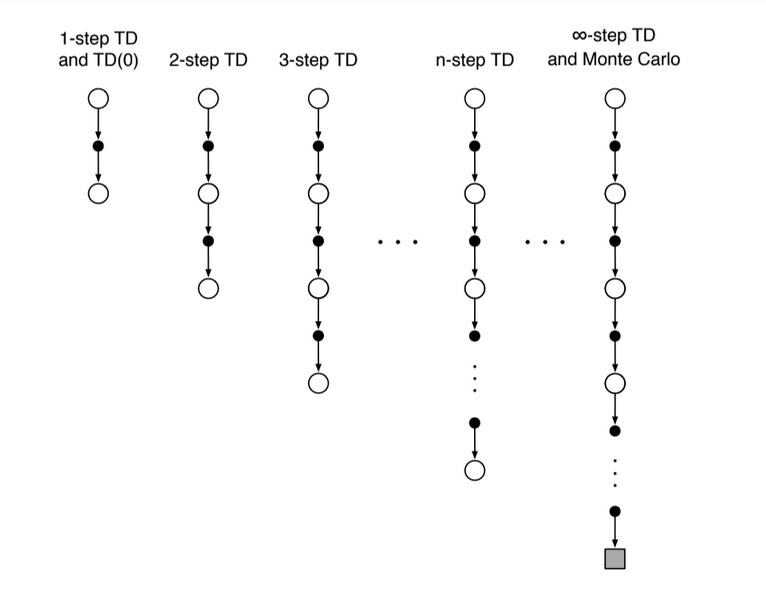
\includegraphics[width=0.8\textwidth]{nstep_diagram.png}}
    \caption{ Backup diagrams for n-step methods }
\end{figure}
Still TD: we bootstrap because we change an earlier estimate based on how it differs from a later estimate (only that the later estimate is now n steps later)

\subsubsection{Targets}

notation: $G_t^{(n)} = G_{t:t+n}$, the return from time step $t$ to $t+n$
\begin{align}
n = 1 & \quad (TD(0)) \quad &  G_t^{(1)} = R_{t+1} + \gamma V_t(S_{t+1}) \label{eq:7.1}\tag{7.1}\\
n = 2 &  &  G_t^{(2)} = R_{t+1} + \gamma R_{t+2} + \gamma^2 V_{t+1}(S_{t+2})\tag{}\\
\vdots &  &  \vdots\tag{}\\
n = \infty & \quad (MC) \quad &  G_t^{(\infty)} = R_{t+1} + \gamma R_{t+2} + ... + \gamma^{T-1} R_T \label{eq:7.2}\tag{7.2}
\end{align}
\begin{itemize}
\item In MC, the target is the return
\item In one-step TD, the target is the one-step return, that is the first reward plus the discounted estimated value of the next state
\item $V_t: \cS \rightarrow \bR$ is the estimate at time $t$ of $v_\pi$.
\end{itemize}

n-step target:
\begin{align}
G_t^{(n)} = R_{t+1} + \gamma R_{t+2} + ... + \gamma^{n-1} R_{t+n} + \gamma^n V_{t+n-1}(S_{t+n}) \label{eq:7.3}\tag{7.3}
\end{align}

\begin{itemize}
\item All n-step returns can be considered approximations of the full return, truncated after n steps and then corrected for the remaining steps by $V_{t+n-1}(S_{t+n})$
\item n-steps return for $n \geq 1$ involve future rewards that are not available from the transition $t \rightarrow t + 1$; we will see eligibility traces for an online method not involving future rewards
\item plugging this into the state-value learning
\end{itemize}
\begin{align}
V_{t+n}(S_t) \doteq V_{t+n-1}(S_t) + \alpha[G_t^{(n)} - V_{t+n-1}(S_t)] \label{eq:7.4}\tag{7.4}
\end{align}
\begin{itemize}
\item no changes are made during the first (n-1) steps of each episode. To make up for that, an equal number of updates are made after the termination of the episode, before starting the next.
\end{itemize}

\begin{figure}[h!]
    \centering
    \subfigure[]{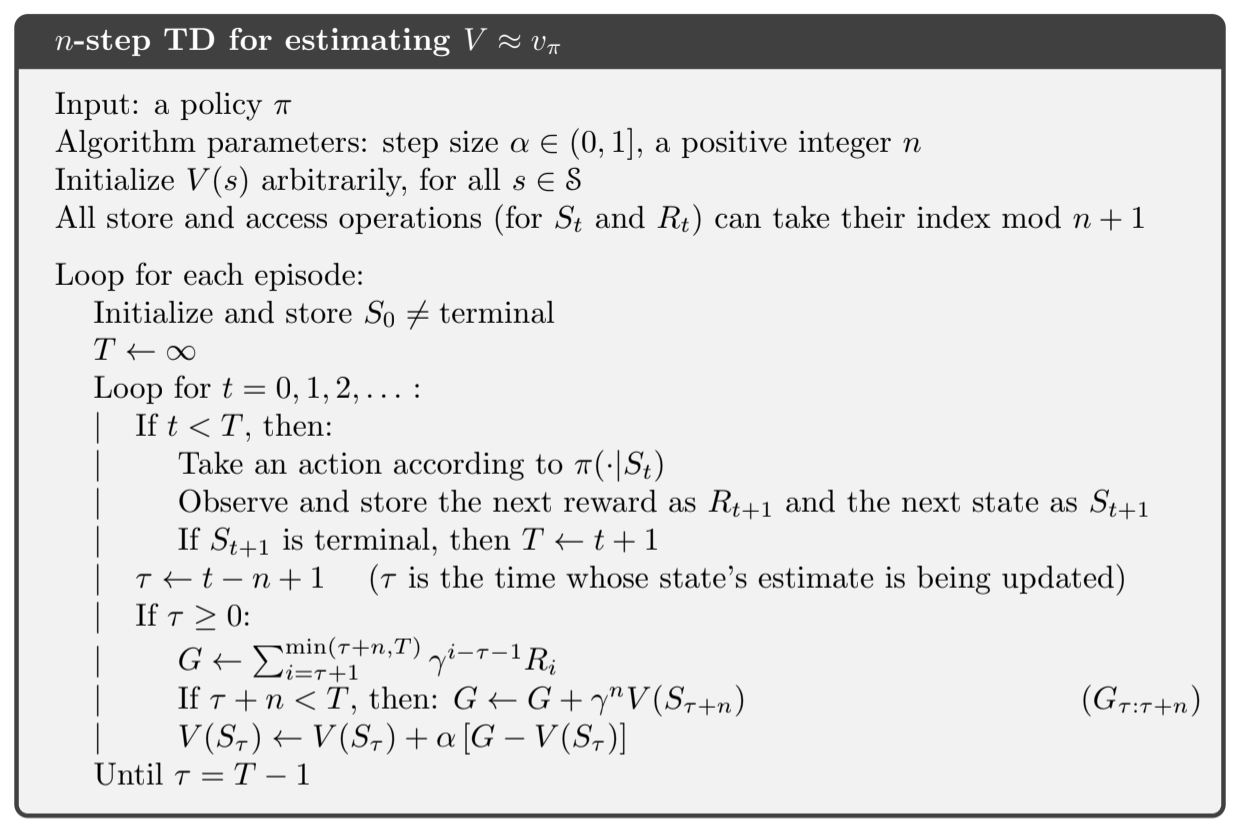
\includegraphics[width=0.8\textwidth]{nstep_algo.png}}
    \caption{ n-step TD algorithm }
\end{figure}

\subsubsection{Error-reduction Property}

The n-step return uses the value function $V_{t+n-1}$ to correct for the missing rewards beyond $R_{t+n}$. An important property of the n-step returns is that their expectation is guaranteed to be a better estimate of $v_\pi$ than $V_{t+n-1}$ is in a worst-state sense.
The worst error of the expected n-step return is guaranteed to be less than or equal to $\gamma^n$ times the worst error under $V_{t+n-1}$.
\begin{align}
\underset{s}{\mathrm{max}} \; | \mathbb{E}_{\pi} [G_t^{(n)} | S_t = s] - v_{\pi}(s) | \leq \gamma^n \underset{s}{\mathrm{max}} \; | V_{t+n-1}(s) - v_{\pi}(s)| \label{eq:7.5}\tag{7.5}
\end{align}
This is called the \textbf{error reduction property}. We can use this to show that all n-steps methods converge to the correct predictions under appropriate technical conditions.

We use this to type of graph to show the effect of n

\begin{figure}[h!]
    \centering
    \subfigure[]{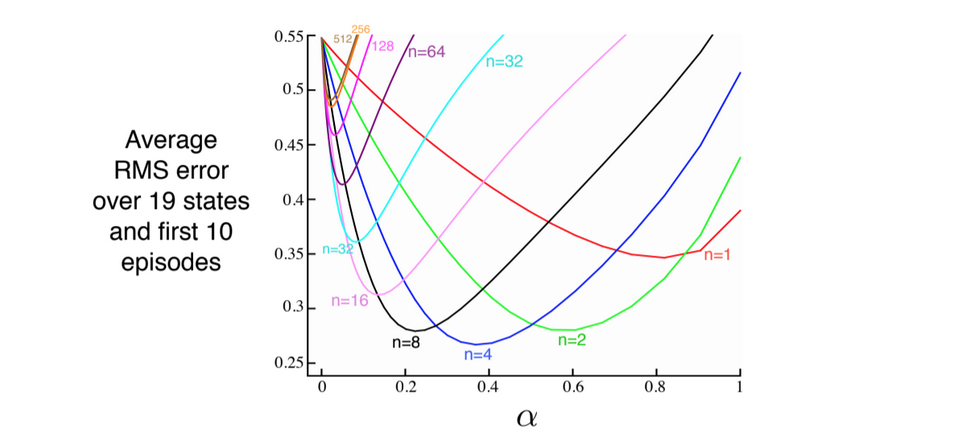
\includegraphics[width=0.8\textwidth]{nstep_graph.png}}
    \caption{ Performance of n-step TD methods as a function of $\alpha$ }
\end{figure}

\newpage
\subsection{n-step SARSA}

\begin{itemize}
\item use n-step not just for prediction but also for control
\item change from states to state-action pairs, and use a $\varepsilon$-greedy policy
\item The backup diagrams for n-step SARSA are like those of n-step TD, except that the SARSA ones start and end in a state-action node.
We redefine the n-step return in terms of estimated action-values instead of state-values
\end{itemize}
\begin{align}
G_{t:t+n} = R_{t+1} + \gamma R_{T+2} + ... + \gamma^{n-1} R_{t+n} + \gamma^n Q_{t+n-1}(S_{t+n}, A_{t+n}) \label{eq:7.6}\tag{7.6}
\end{align}
\begin{itemize}
\item and plug that into our GPI update
\end{itemize}
\begin{align}
Q_{t+n}(S_t, A_t) \gets Q_{t+n-1}(S_t, A_t)  + \alpha \big(G_{t:t+n} - Q_{t+n-1}(S_t, A_t)\big) \label{eq:7.7}\tag{7.7}
\end{align}
The values of all other states remain unchanged, $Q_{t+n}(s,a) = Q_{t+n-1}(s,a)$ for $s \neq S_t$ or $a \neq A_t$.

\begin{figure}[h!]
    \centering
    \subfigure[]{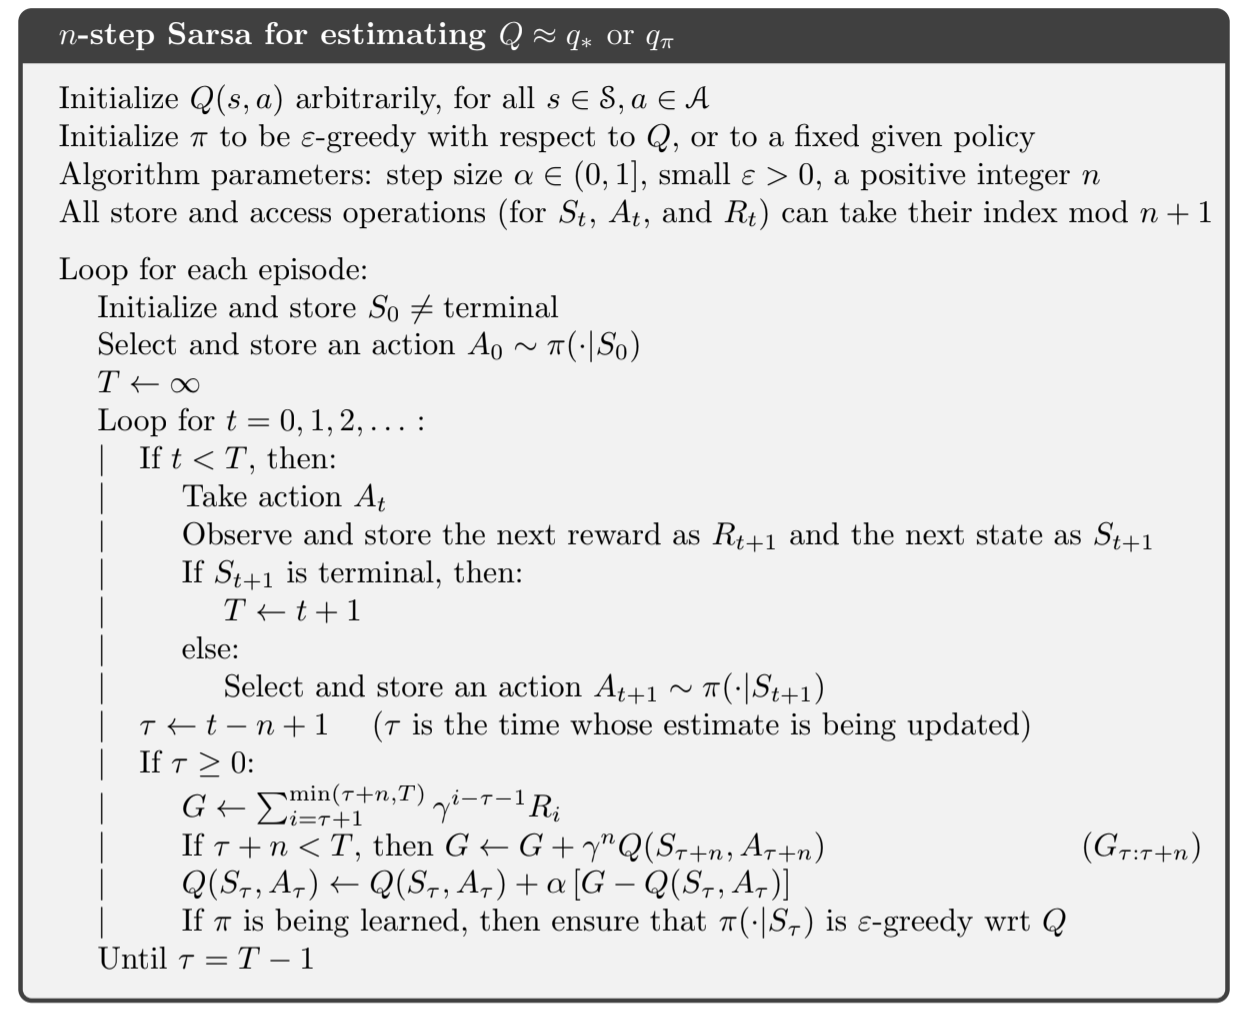
\includegraphics[width=0.8\textwidth]{nstep_sarsa_algo.png}}
    \caption{ n-step SARSA }
\end{figure}
\begin{figure}[h!]
    \centering
    \subfigure[]{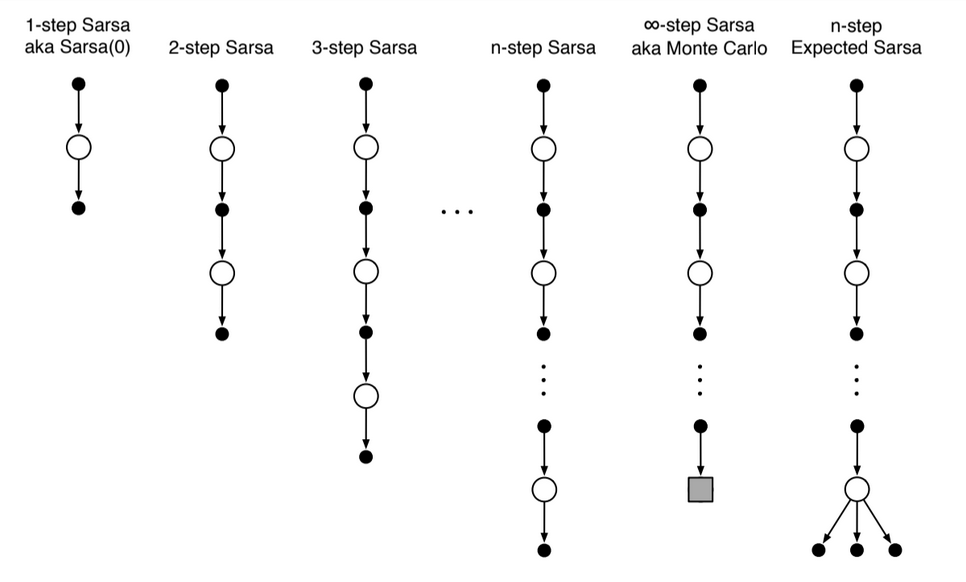
\includegraphics[width=0.8\textwidth]{nstep_sarsa.png}}
    \caption{ n-step SARSA backup diagram }
\end{figure}

\subsubsection{Expected SARSA}

What about n-step version of expected SARSA? The backup diagram consists of a linear string of sample actions and states and the last element is a branch over all action possibilities, weighted by their probability of occurring under $\pi$. The n-step return is here defined by:
\begin{align}
G_{t:t+n} = R_{t+1} + \gamma R_{T+2} + ... + \gamma^{n-1} R_{t+n} + \gamma^n \bar{V}_{t+n-1}(S_{t+n}, A_{t+n}) \label{eq:7.8}\tag{7.8}
\end{align}
Where $\bar{V_t}(s)$ is the expected approximate value of state $s$, using the estimated action values and the policy
$$ \bar{V_t}(s) \doteq \sum_a \pi(a|s)Q_t(s,a) $$
\begin{itemize}
\item Expected approximate values are important!
\item if $s$ is terminal, then its approximated value is defined to be 0.
\end{itemize}

\subsection{n-step Off-policy Learning (by importance sampling)}

\begin{itemize}
\item To use the data from behavior policy $b$, we must take into account the relative probability of taking the actions that were taken
\item In n-step methods, the returns are constructed over $n$ steps so we are interested in the relative probability of just these $n$ actions
\end{itemize}

For example, to make a simple version of $n$-step TD, we can weight the update for time $t$ (made at time $t+n$) by the importance sampling ratio
\begin{align}
\rho_{t:h} = \prod_{k=t}^{min(h, T-1)} \frac{\pi(A_k\|S_k)}{b(A_k\|S_k)} \label{eq:7.10}\tag{7.10}
\end{align}
If we plug this into our update, we get
$$ V_{t+n}(S_t) \gets V_{t+n-1}(S_t)  + \alpha \rho_{t:t+n-1} (G_{t:t+n} - V_{t+n-1} (S_t)) $$
Similarly, the n-step SARSA update can be extended for the off-policy method
$$Q_{t+n}(S_t, A_t) \gets Q_{t+n-1}(S_t, A_t)  + \alpha \rho_{t+1:t+n-1} (G_{t:t+n} - Q_{t+n-1}(S_t, A_t)) $$

Note that the IS ratio here starts one step later than from $n$-step TD because we are updating a state-action pair (we know that we have selected the action so we need IS only for the subsequent actions).

\begin{figure}[h!]
    \centering
    \subfigure[]{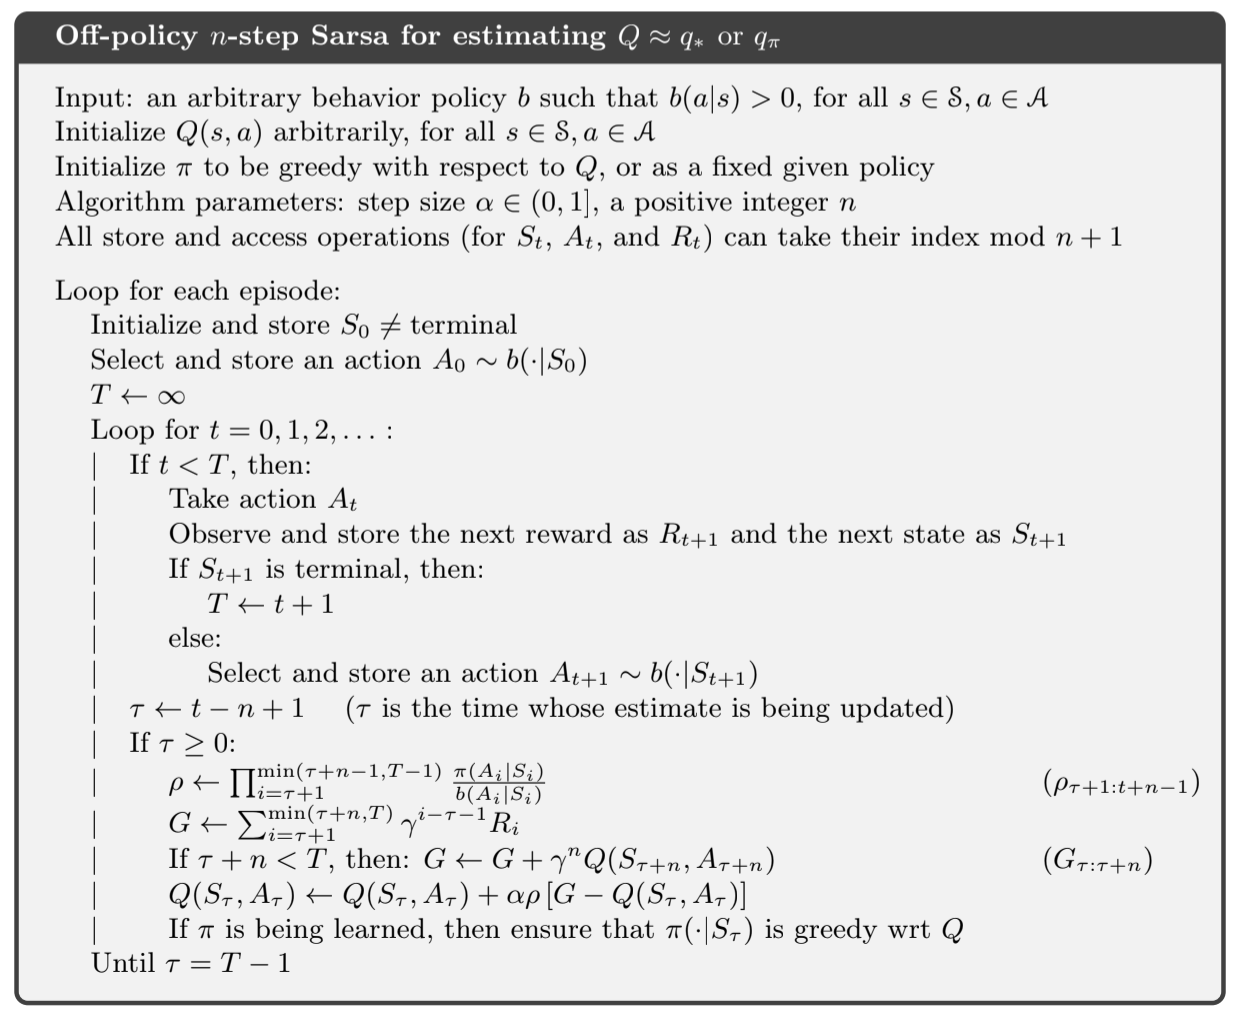
\includegraphics[width=0.8\textwidth]{nstep_sarsa_offpolicy.png}}
    \caption{ n-step SARSA off-policy algorithm }
\end{figure}

The off-policy version for \textbf{expected SARSA} would be the same except that the IS ratio would use $\rho_{t+1:t+n-2}$ instead of $\rho_{t+1:t+n-1}$ because all possible actions are taken into account $\textit{in the last state}$, the one actually taken has no effect and does not need to be corrected for.

\textbf{why Q-learning can be off-policy w/o IS?}

Q-learning bootstraps off of the largest action value in its next state. This is like sampling an action under an estimate of the optimal policy rather than the behavior policy. Q-learning learns about the best action it could take rather the actions it actually takes, so it's off-policy.

\textbf{why expected SARSA can be off-policy w/o IS?}

the expectation over actions is computed independently of the action actually selected in the next state, so it's off-policy

\textbf{why Q-learning doesn't use IS?}

\url{https://stats.stackexchange.com/questions/335396/why-dont-we-use-importance-sampling-for-one-step-q-learning}
For action values, the fist action does not play a role in the IS ratio (it has been taken!).


\subsection{Per-decision Methods with Control Variates}

The multi-step off-policy methods presented in 7.3 is conceptually clear but not very efficient. What about per-decision sampling (recall Chap 5.9).

1. The n-step return can be written recursively. For the $n$ steps being ending at horizon $h$, the $n$-step return can be written $G_{t:h} = R_{t+1} + \gamma R_{t+1:h}$

2. Consider the effect of following behavior policy $b$ is not the same as following policy $\pi$, so all the resulting experiences, including the first reward $R_{t+1}$ and the next state $S_{t+1}$, must be weight by the importance sampling ratio for time $t$, $\rho_t = \frac{\pi(A_t|S_t)}{b(A_t|S_t)}$

A simple approach would be to weight the right-hand side $R_{t+1}+\gamma G_{t+1:h}$ by $\rho_t$. A more sophisticated approach would be to use an off-policy definition of the $n$-step return ending in horizon $h$
\begin{align}
G_{t:h} \doteq \rho_t(R_{t+1} + \gamma G_{t+1:h}) + (1 - \rho_t) V_{h-1}(S_t) \label{eq:7.11}\tag{7.11}
\end{align}
where $t < h < T$, and $G_{h:h} \doteq V_{h-1} (S_h)$.

If $\rho_t = 0$ (trajectory has no chance to occur under the target policy), then instead of changing the target $G_{t:h}$ to be 0 and causing the estimate to shrink, the target is the same as the estimate and cause no change. The additional term $(1 - \rho_t) V_{h-1}(S_t)$ is called a \textbf{control variate} and conceptually is here to ensure the idea that if $\rho_t = 0$, then we should ignore the sample and don't change the estimate.

We can otherwise use the conventional learning rule that does not have explicit IS ratios, except the one in $G_{t:h}$.

\subsubsection{For action values}

For action values, the off-policy definition of the $n$-step return is a little different because the first action does not play a role in the IS ratio (it has been taken!).

The $n$-step on-policy return ending at horizon $h$ can be written recursively, and for action-values, the recursion ends with $G_{h:h}\doteq \bar{V_{h-1}}(S_h)$. An off-policy form with control variate is:
\begin{align}
G_{t:h} & \doteq R_{t+1} + \gamma \big(\rho_{t+1} G_{t+1:h} + \bar{V}_{h-1}(S_{t+1}) - \rho_{t+1} Q_{h-1}(S_{t+1}, A_{t+1}) \big) \label{eq:7.12}\tag{7.12}\\
 & = R_{t+1} + \gamma \rho_{t+1}\big(G_{t+1:h} Q_{h-1}(S_{t+1}, A_{t+1}) \big) + \gamma \bar{V}_{h-1}(S_{t+1}) \big)\label{eq:7.13}\tag{7.13}
\end{align}
for $t < h < T$.
\begin{itemize}
\item if $h < T$, then the recursion end with $G_{h:h} \doteq (S_h, A_h)$
\item if $h = T$, it ends with $G_{T-1:T} \doteq R_T$. The resultant prediction algorithm is analogous to Expected SARSA.
\end{itemize}

\textbf{Off-policy methods have higher variance} and it's probably inevitable. Things to help reduce the variance:
\begin{itemize}
\item control variates
\item adapt the step size parameter to the observed variance
\item invariant updates
\end{itemize}

\subsection{Off-policy Learning Without Importance Sampling: The n-step Tree Backup Algorithm}

Off-policy without IS: Q-learning and Expected SARSA do it for the one-step case. Here, we present a multi-step algorithm: \textbf{the tree backup algorithm}.

\begin{figure}[h!]
    \subfigure[]{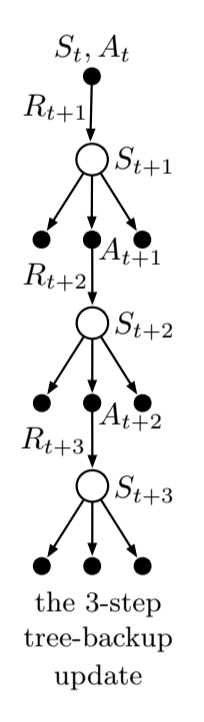
\includegraphics[width=0.1\textwidth]{nstep_tree.png}}
    \caption{ n-step tree }
\end{figure}
A 3-step tree backup diagram
\begin{itemize}
\item 3 sample states and rewards
\item 2 sample actions
\item list of unselected actions for each state
\item we have no sample for the unselected actions, and we bootstrap with their estimated values
\end{itemize}

So far, the target for the update of a node was combining the rewards along the way and the estimated values of the nodes at the bottom. Now we add to this the estimated values of the actions not selected. This is why it is called a tree backup update: it is an update from the entire tree of estimated action values.

Each leaf node contributes to the target with a weight proportional to their probability of occurring under $\pi$.
\begin{itemize}
\item each first-level action $a$ contributes with a weight of $\pi(a|S_{t+1})$
\item the action actually taken, $A_{t+1}$, does not contribute and its probability $\pi(A_{t+1} | S_{t+1})$ is used to weight all the second level action values
\item each second-level action $a'$ thus has a weight of $\pi(A_{t+1} | S_{t+1}) \pi (a' | S_{t+2})$
\end{itemize}
The one-step return (target) is the same as Expected SARSA (for $t < T - 1$):
\begin{align*}
G_{t:t+1} \doteq R_{t+1} + \gamma \sum_a \pi(a| S_{t+1}) Q_t(S_{t+1}, a) \label{eq:7.14}\tag{7.14}
\end{align*}
And the two-step tree-backup return is (for $t < T - 2$):
\begin{equation} \label{eq4}
\begin{split}
G_{t:t+2} & \doteq R_{t+1} + \gamma \sum_{a \neq A_{t+1}} \pi(a| S_{t+1}) Q_t(S_{t+1}, a) \\
& + \gamma \pi(A_{t+1}|S_{t+1}) \big(R_{t+2} + \gamma \sum_a \pi(a|S_{t+2}) Q_{t+1}(S_{t+2}, a)\big)\\
 & = R_{t+1} + \gamma \sum_{a \neq A_{t+1}} \pi(a| S_{t+1}) Q_t(S_{t+1}, a) + \gamma \pi(A_{t+1}|S_{t+1}) G_{t+1:t+2}
\end{split}
\end{equation}
The latter form suggests the recursive form of the n-step tree backup return (for $t < T - 1$):
\begin{align}
G_{t:t+n} \doteq R_{t+1} + \gamma \sum_{a \neq A_{t+1}} \pi(a| S_{t+1}) Q_{t+n-1}(S_{t+1}, a) + \gamma \pi(A_{t+1}|S_{t+1}) G_{t+1:t+n} \label{eq:7.15}\tag{7.15}
\end{align}
We then use this target in the usual action-value update from n-step SARSA:
\begin{align}
Q_{t+n}(S_t, A_t) \gets Q_{t+n-1}(S_t, A_t)  + \alpha \big(G_{t:t+n} - Q_{t+n-1}(S_t, A_t)\big) \label{eq:7.16}\tag{7.16}
\end{align}

\begin{figure}[h!]
    \centering
    \subfigure[]{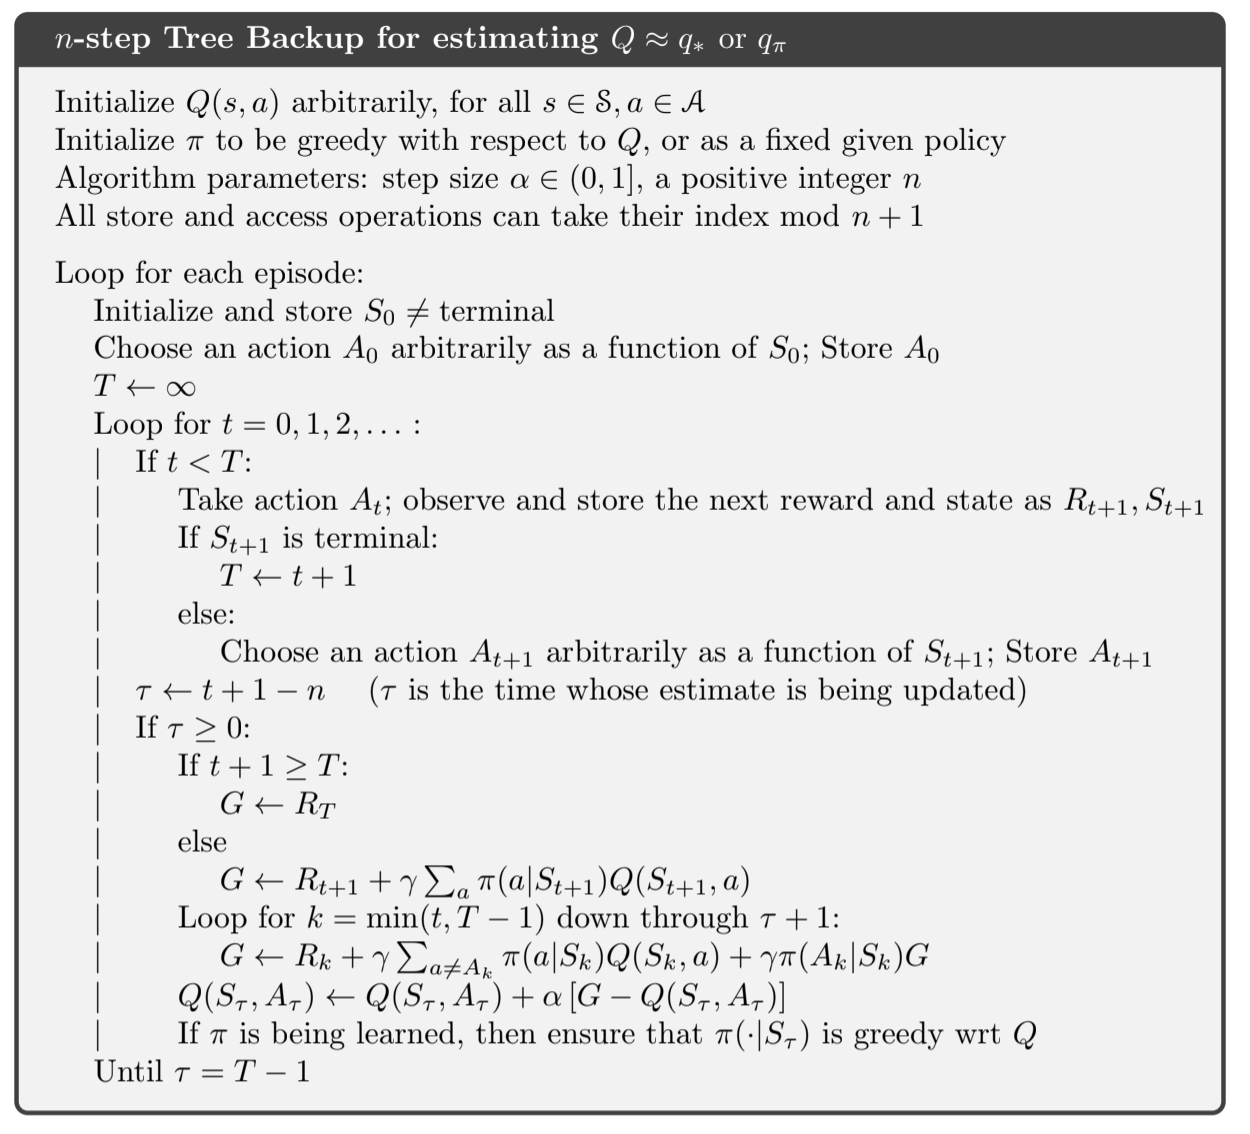
\includegraphics[width=0.8\textwidth]{nstep_tree_backup.png}}
    \caption{ n-step tree backup algorithm }
\end{figure}

\newpage
\subsection{A Unifying Algorithm: n-step Q($\sigma$)}

So far we have considered 3 different kinds of action-value algorithms, the first 3 of the figure:
\begin{figure}[h!]
    \centering
    \subfigure[]{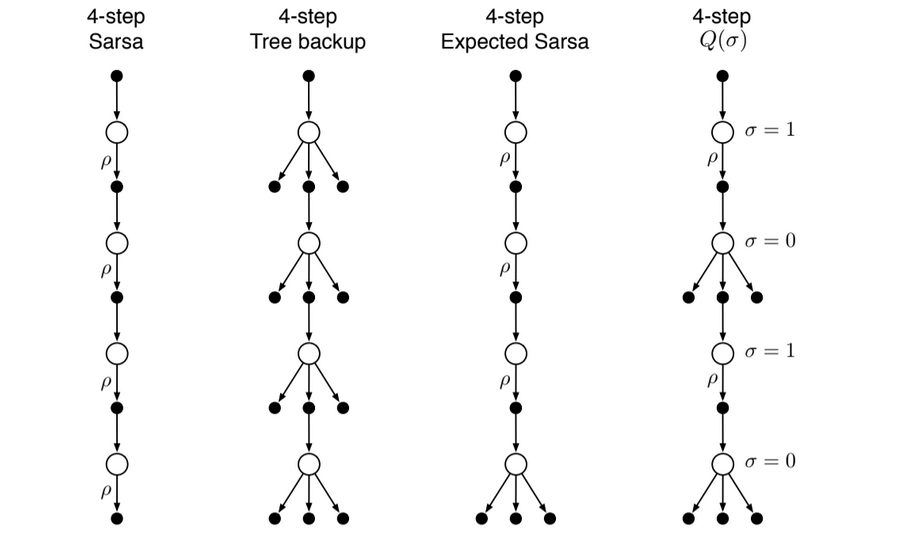
\includegraphics[width=0.8\textwidth]{nstep_diagrams.png}}
    \caption{ n-step backup diagrams. The $rho$'s indicate half transitions on which IS is required in the off-policy case }
\end{figure}
\begin{itemize}
\item n-step SARSA has all sample transitions
\item the tree backup has all state-to-action transitions branched w/o sampling
\item n-step Expected SARSA has all sample transitions except for the last state which is fully branched with an expected value
\end{itemize}

Unification algorithm: last diagram.

Basic idea: decide on a step-by-step basis whether we want to sample as in SARSA or consider the expectation over all the actions instead, as in the tree backup update.

\begin{itemize}
\item let $\sigma_t \in [0,1]$ denote the degree of sampling on step $t$, 1 = full sampling, 0 = taking expectation
\item the random variable $\sigma_t$ might be set as a function of (s) or (s,a) at time $t$
\end{itemize}

This algorithm is called $n$-step Q($\sigma$). To develop its equations, first we need to write the tree-backup $n$-step return in terms of the horizon $h = t + n$ and the expected approximate value $\bar{V}$:
\begin{align*}
G_{t:h} & \doteq R_{t+1} + \gamma \sum_{a \neq A_{t+1}} \pi(a| S_{t+1}) Q_{h-1}(S_{t+1}, a) + \gamma \pi(A_{t+1}|S_{t+1}) G_{t+1:h}\\
 & = R_{t+1} + \gamma \bar{V}_{h-1}(S_{t+1}) - \gamma \pi(A_{t+1} | S_{t+1}) - Q_{h-1}(S_{t+1}, A_{t+1}) + \gamma \pi(A_{t+1}|S_{t+1})G_{t+1:h}\\
 & = R_{t+1} + \gamma \pi(A_{t+1} | S_{t+1}) \big( G_{t+1:h} - Q_{h-1}(S_{t+1}, A_{t+1})\big) + \gamma \bar{V}_{h-1}(S_{t+1}) \label{eq:7.17}\tag{7.17}
\end{align*}
After which this is exactly like the $n$-step return for SARSA with Control Variates, except with the action probability $\pi(A_{t+1} | S_{t+1})$ substituted for the IS ratio $\rho_{t+1}$. For Q($\sigma$), we slide linearly between these two cases
\begin{align*}
G_{t:h} \doteq R_{t+1} + \gamma\big(\sigma_{t+1} \rho_{t+1} + (1 - \sigma_{t+1})\pi(A_{t+1}|S_{t+1})\big)\big( G_{t+1:h} - Q_{h-1}(S_{t+1}, A_{t+1})\big) \\+ \gamma \bar{V}_{h-1}(S_{t+1})s
\end{align*}
for $t < h \leq T$. The recursion ends with $G_{h:h} \doteq 0$ if $h < T$or with $G_{T-1:T} = R_T$ if $h = T$

Once this return is well defined, we can plug it into the usual $n$-step SARSA upate.

\begin{figure}[h!]
    \centering
    \subfigure[]{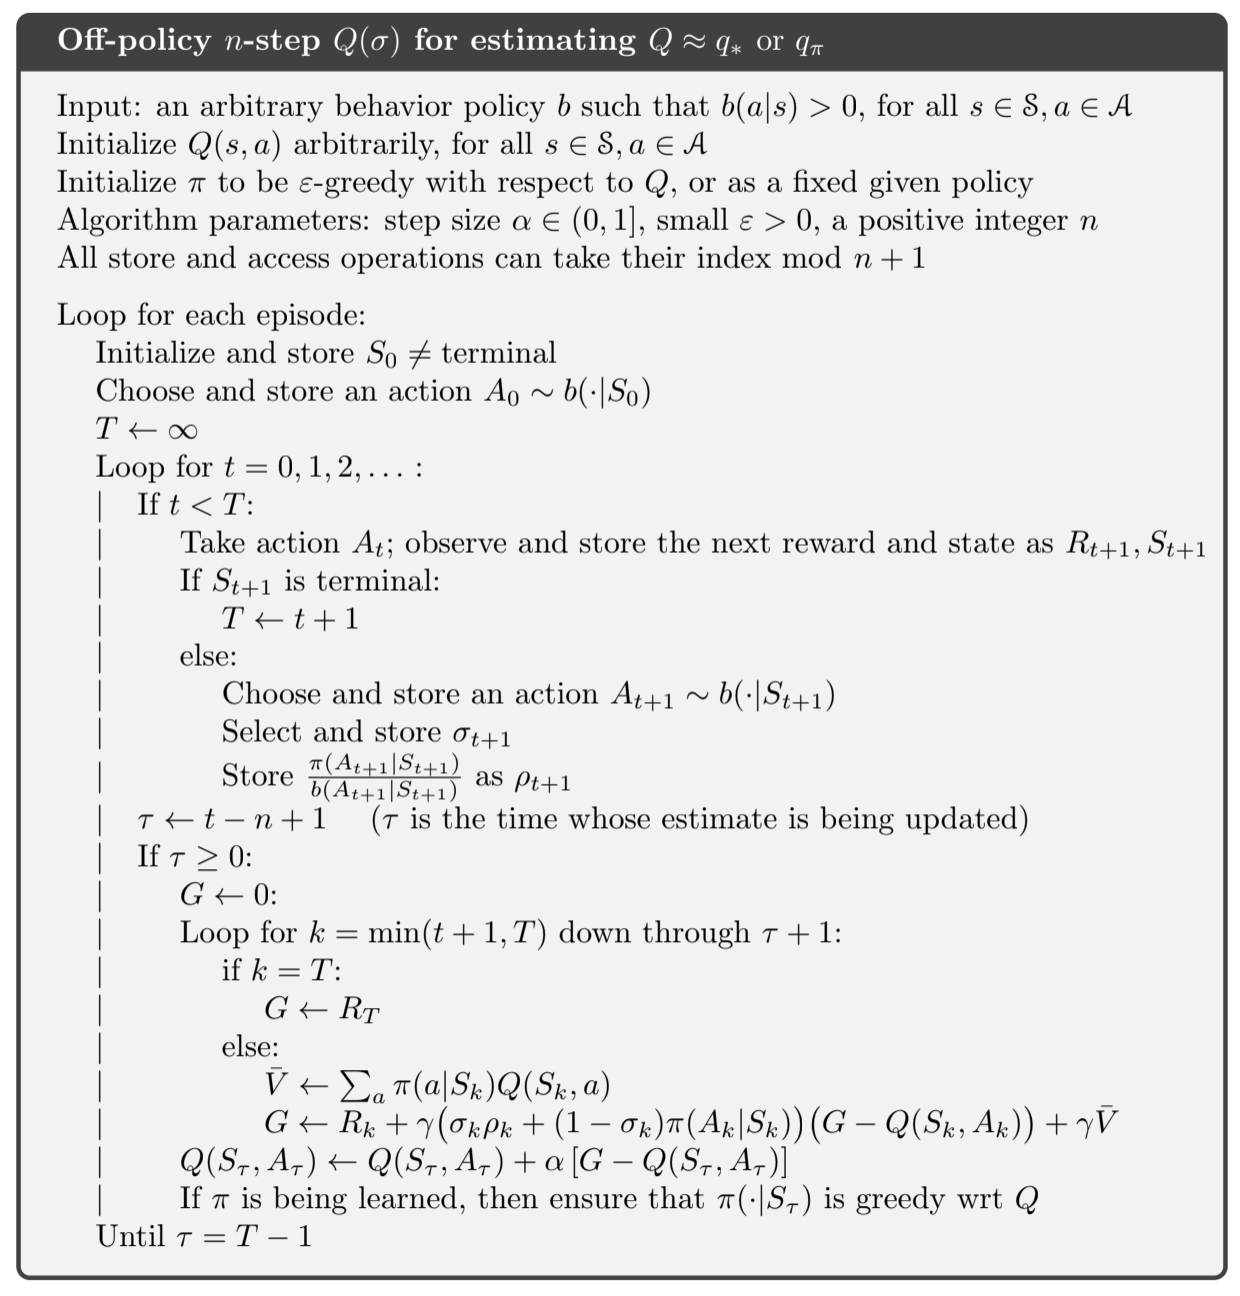
\includegraphics[width=0.8\textwidth]{nstep_qsigma.png}}
    \caption{ n-step Q($\sigma$) }
\end{figure}

\newpage
\subsection{Summary}

\begin{itemize}
\item Range of TD methods between one-step TD and MC methods
\item $n$-step methods look ahead to the next $n$ rewards, states and actions
\item all $n$-step methods require a delay of $n$ steps before updating (because we need to know what happens in the next $n$ steps) -> Eligibility Traces :)
\item they also involve more computation than previous one-step methods (it's worthwhile, since one-step methods are limited)
\item two approaches for off-policy learning have been explained:
\begin{itemize}
	\item with importance sampling. Simple but high variance
	\item tree-backup updates (no IS). A natural extension of Q-learning to multi-step case with stochastic target policies
\end{itemize}
\end{itemize}

\end{document}